\section{How it's different from Word}
\subsection{WYSIWYG - What You See Is What You Get}
You may be familiar with the challenge that is using Word to write equations even as simple as those in Figure \ref{fig:word}.
The formatted text on the page is exactly everything you have, which often means spending time trying to fix how it looks and what goes where, a process we call typesetting. So \textbf{what is the alternative?}

\begin{figure}
    \centering
    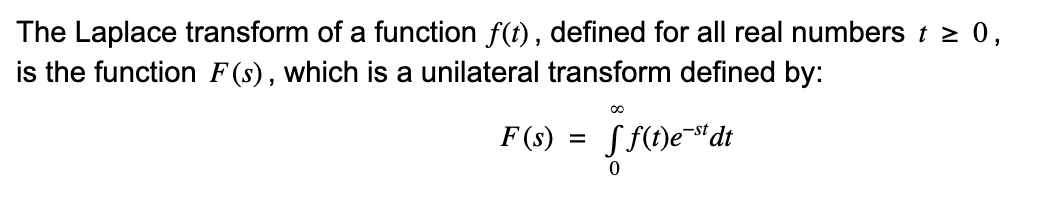
\includegraphics[scale=0.8]{figures/word.png}
    \caption{Word, an example of What You See Is What You Get}
    \label{fig:word}
\end{figure}

\pagebreak

\subsection{Typesetting}
Let me introduce you to \LaTeX, pronounced either \emph{lah-tec} or \emph{lay-tec}.

-- \textbf{stuff here}.

The main motivators for why you would want to use it are:
\begin{enumerate}
    \item Beautifully written documents. No more trying to deal with the various fonts, margins, spacing, etc.;
    \item Easy bibliography management, citations and cross-references;
    \item Easy equations and graphs. Even extremely complicated mathematical concepts can be easily written.
\end{enumerate}

Let's go back to our example, and see how it would be done with \LaTeX:
\lstinputlisting[language=TeX, label=ls:Laplace, caption=Example document written with \LaTeX]{files/lesson-plan/introduction/example1.tex}

If you are familiar with programming, this may vaguely look like a \emph{markup language}, and it is!
If you are not, don't worry. We will introduce the most distinctive features, and go into more detail as necessary.

\subsection{Markup language}
There are generally three types of markups:
\begin{enumerate}
    \item \textbf{Environments} introduce some kind of formatting, such as lists, math mode or more complicated things. A backslash, \verb|\|, is used to indicate a markup, curly brackets \verb|{}| indicate an \emph{argument}, and square brackets \verb|[]| (optionally) provide options.
    
    With very few exceptions, environments have the following format:
    
    \begin{lstlisting}
    \begin{environment-name}[options]
        ...
    \end{environment-name}
    \end{lstlisting}
    
    One of the exceptions is in Listing \ref{ls:Laplace}. Can you spot it? It is \verb|$...$|, the \emph{in-line math mode} environment. We will be exploring it in more detail later.

    \item \textbf{Instructions} define some feature of the document. This ranges from breaking a page to defining the  headings you have available. In our example you can see:

    \verb|\documentclass[...]{article}|
    
    \item \textbf{Variables} can either be predefined or user defined, and these range from greek letters to the integral sign to a whole expression.
    Some examples seen are \verb|\geq| (\textbf{g}reater or \textbf{eq}ual) and \verb|\int| ($\int$). Intuitively, \verb|\alpha| results in $\alpha$, and similarly for other greek letters.  
    
    \textbf{Note:} There are some characters with predefined meaning, such as \verb|{|, \verb|}| and \verb|&|. To use the literal curly brackets, ampersand, etc we would need to \emph{escape} them. Conveniently, this is done with a backslash (\verb|\|), so feel free to think of it as a variable: \verb|\{|, \verb|\}| and \verb|\&|.
\end{enumerate} 

\subsection{Packages}
    You may have noticed that \verb|\usepackage{amsmath}| was not mentioned as an instruction the previous section. That's because packages are worth mentioning on their own.

    Packages add features to our document, similar to \emph{import} in most programming languages.
    \verb|amsmath| gives us a wide array of maths tools, but there are packages for drawing, graphing, colouring, better management of bibliography, easier organisation of your files\dots and the list goes on.
    
\subsection{Compilation}
    We can use any text editing software to write and save our documents in \verb|.tex| files. In order to produce a \verb|.pdf|, it needs to be \emph{compiled}.
    As a beginner you may spend a lot of time scratching your head, wondering why it's not compiling.
    
    The good news is that recommended IDEs (\textbf{I}ntegrated \textbf{D}evelopment \textbf{E}nvironments, basically text editors filled with features) handle the compilation for you and have features to help you spot mistakes.